\documentclass[./main.tex]{subfiles}

\begin{document}
\section{Dataset}
To perform the pose estimation in Section \ref{sec:experiments}, we need some data on which to train, validate and test our models. The following section describes the datasets that will be used, as well as the preprocessing of these datasets.

\begin{table}[htbp]
    \begin{tabular}{|l|c|c|c|c|}
        \hline
        \multicolumn{1}{|c|}{\textbf{Keypoints}} & \begin{tabular}[c]{@{}c@{}}\textbf{ClimbAlong}\\ \textbf{25 keypoints}\end{tabular} & \begin{tabular}[c]{@{}c@{}}\textbf{ClimbAlong}\\ \textbf{17 keypoints}\end{tabular} & \textbf{BRACE} & \textbf{Penn Action} \\ \hline
        Head & No & No & No & Yes \\ \hline
        Nose & Yes & Yes & Yes & No \\ \hline
        Left ear & Yes & Yes & Yes & No \\ \hline
        Right ear & Yes & Yes & Yes & No \\ \hline
        Left eye & No & Yes & Yes & No \\ \hline
        Right eye & No & Yes & Yes & No \\ \hline
        Left shoulder & Yes & Yes & Yes & Yes \\ \hline
        Right shoulder & Yes & Yes & Yes & Yes \\ \hline
        Left elbow & Yes & Yes & Yes & Yes \\ \hline
        Right elbow & Yes & Yes & Yes & Yes \\ \hline
        Left wrist & Yes & Yes & Yes & Yes \\ \hline
        Right wrist & Yes & Yes & Yes & Yes \\ \hline
        Left pinky & Yes & No & No & No \\ \hline
        Right pinky & Yes & No & No & No \\ \hline
        Left index & Yes & No & No & No \\ \hline
        Right index & Yes & No & No & No \\ \hline
        Left thumb & Yes & No & No & No \\ \hline
        Right thumb & Yes & No & No & No \\ \hline
        Left hip & Yes & Yes & Yes & Yes \\ \hline
        Right hip & Yes & Yes & Yes & Yes \\ \hline
        Left knee & Yes & Yes & Yes & Yes \\ \hline
        Right knee & Yes & Yes & Yes & Yes \\ \hline
        Left ankle & Yes & Yes & Yes & Yes \\ \hline
        Right ankle & Yes & Yes & Yes & Yes \\ \hline
        Left heel & Yes & No & No & No \\ \hline
        Right heel & Yes & No & No & No \\ \hline
        Left toes & Yes & No & No & No \\ \hline
        Right toes & Yes & No & No & No \\ \hline
    \end{tabular}
    \caption{Overview of the annotated keypoints of the four used datasets}
    \label{tab:keypoints}
\end{table}

\subsection{The ClimbAlong Dataset}
\begin{figure}[htbp]
    \centering
    \begin{subfigure}{0.3\textwidth}
        \centering
        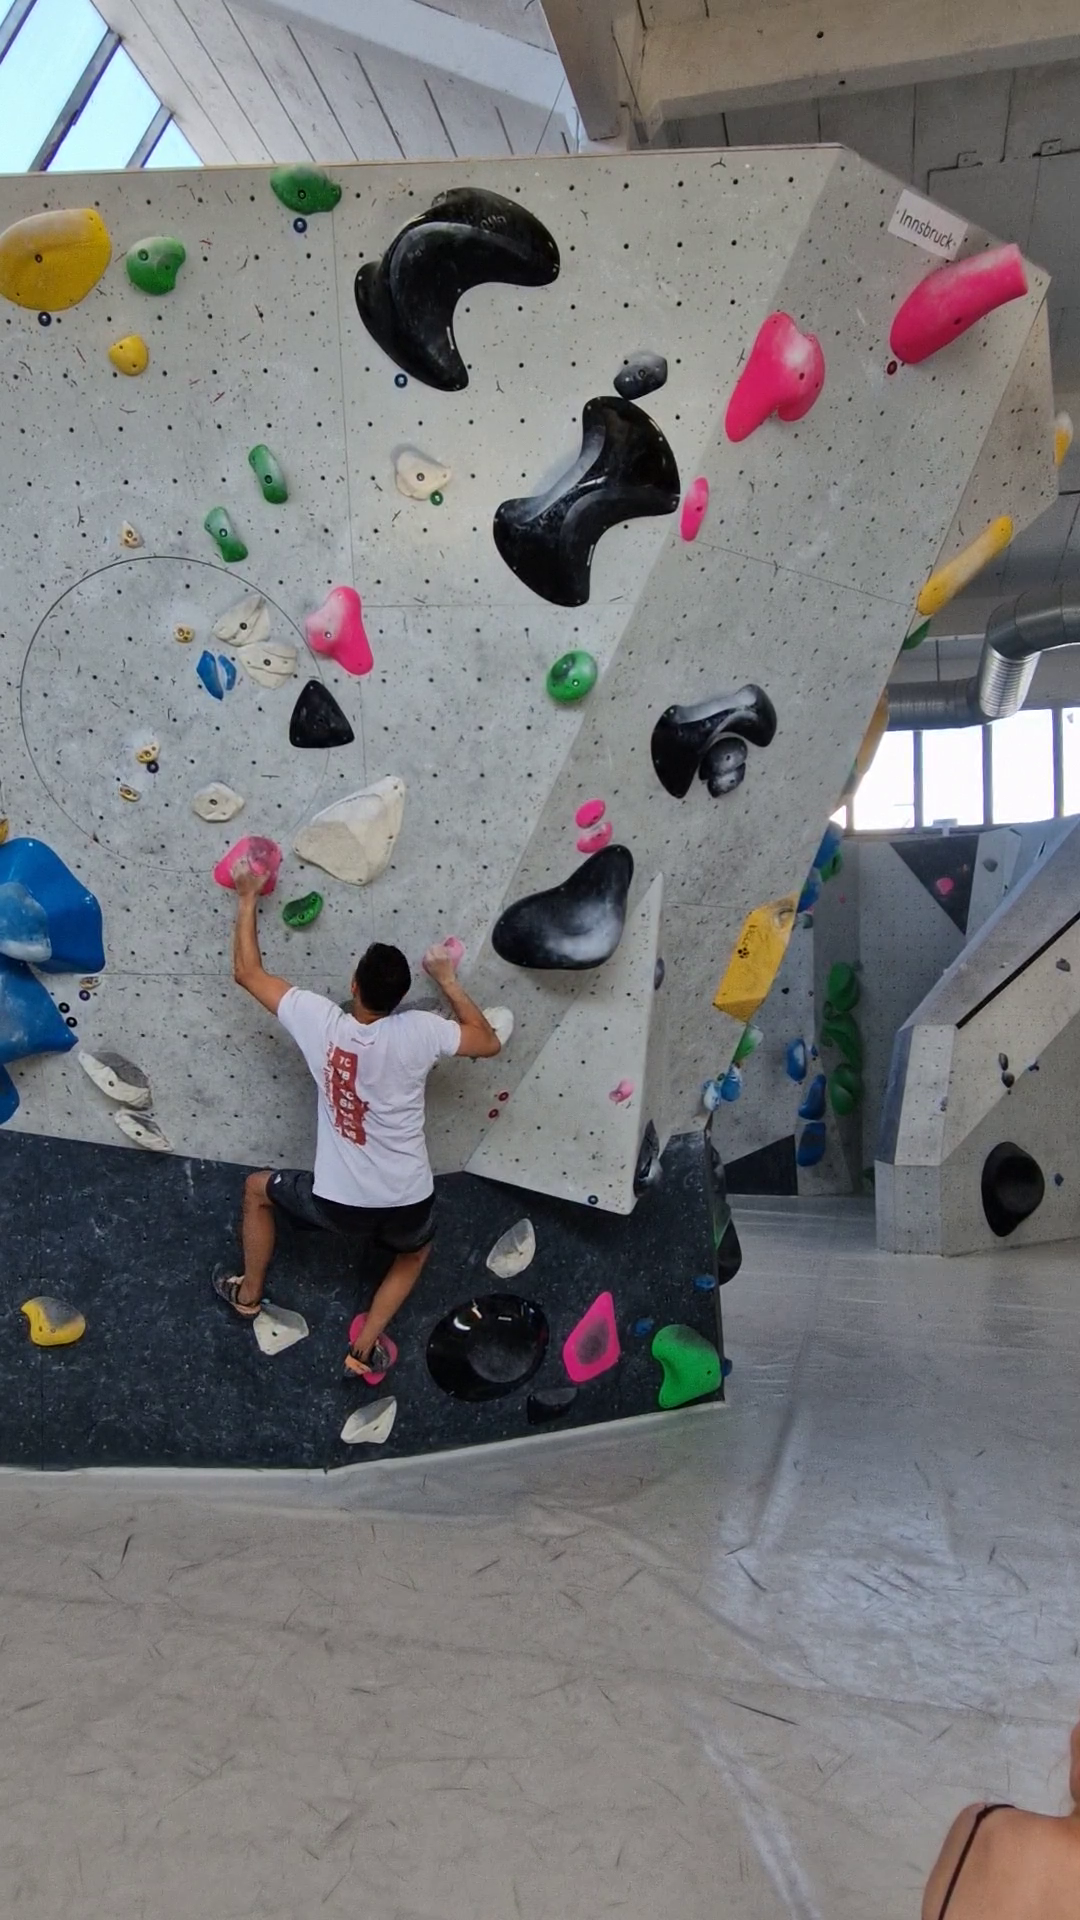
\includegraphics[width=\textwidth]{entities/CA_262.png}
        \caption{Frame 262}
    \end{subfigure}
    \begin{subfigure}{0.3\textwidth}
        \centering
        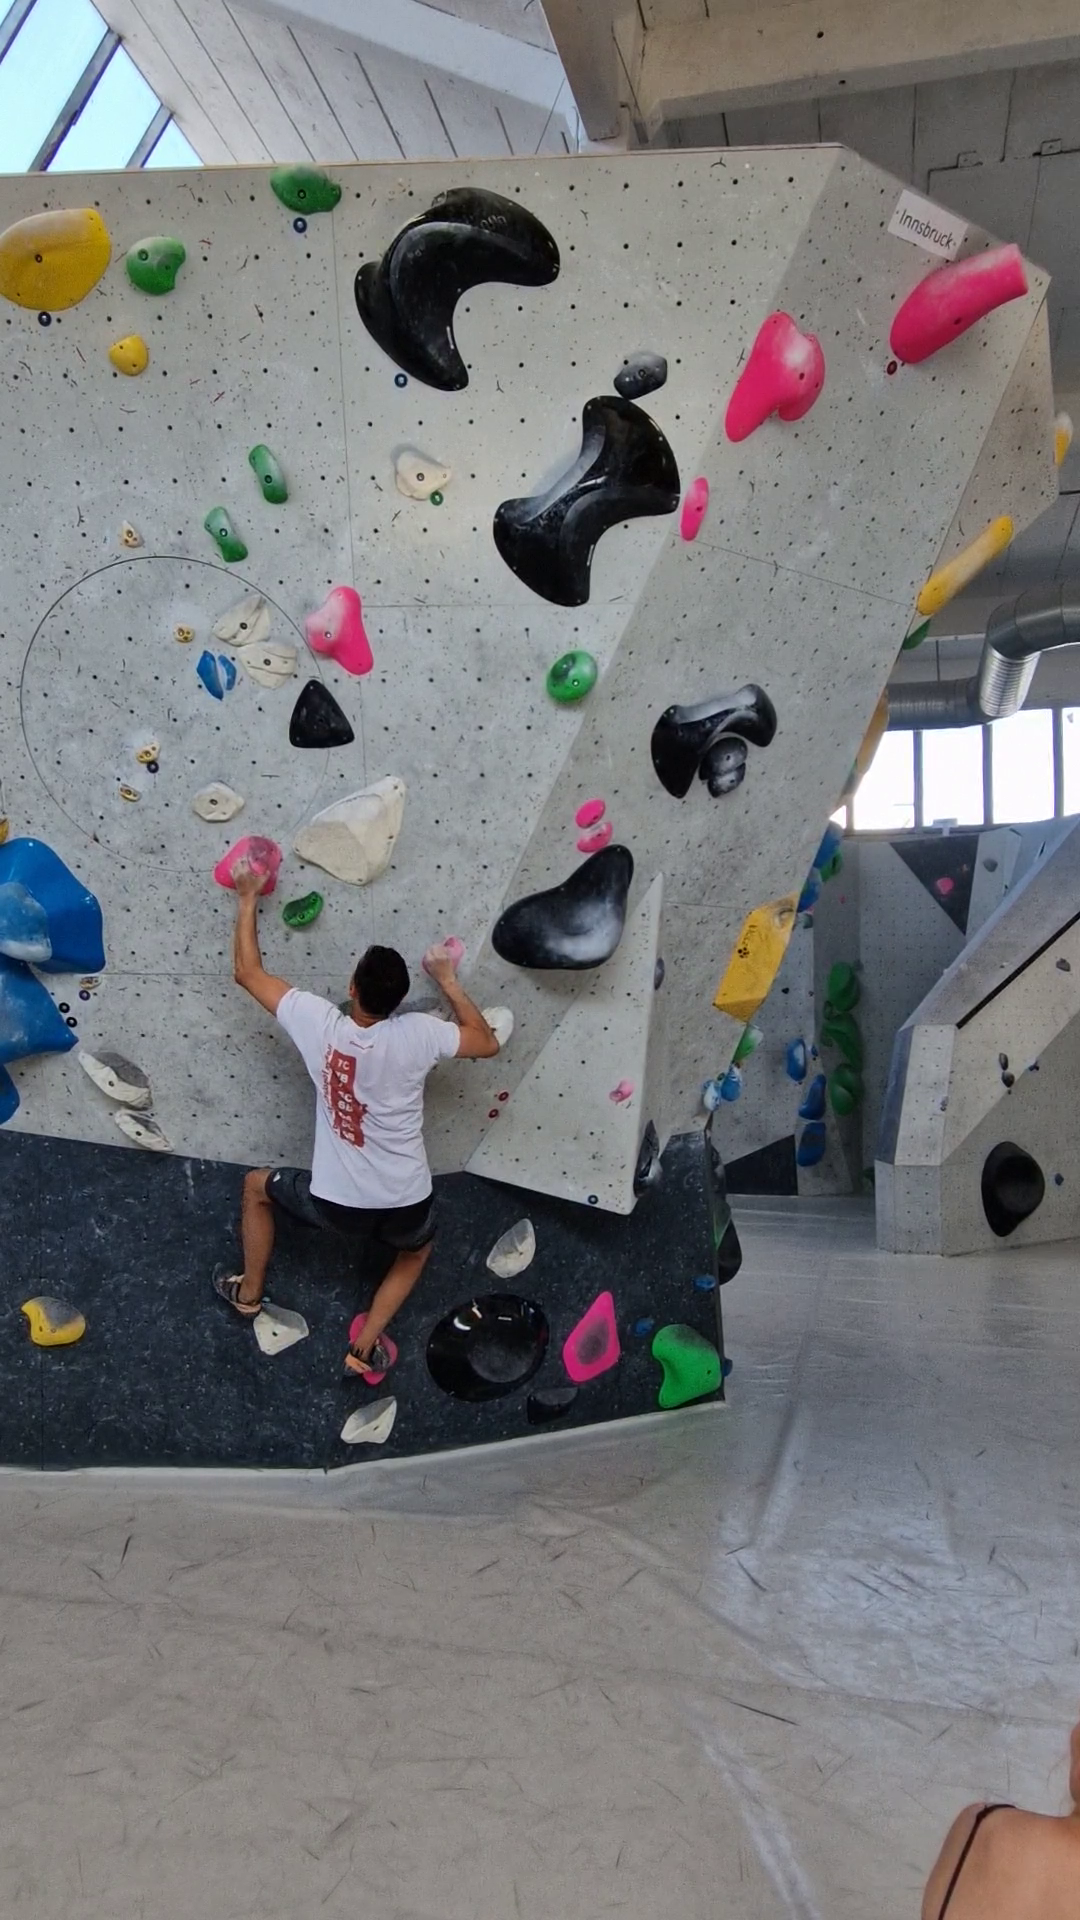
\includegraphics[width=\textwidth]{entities/CA_263.png}
        \caption{Frame 263}
    \end{subfigure}
    \begin{subfigure}{0.3\textwidth}
        \centering
        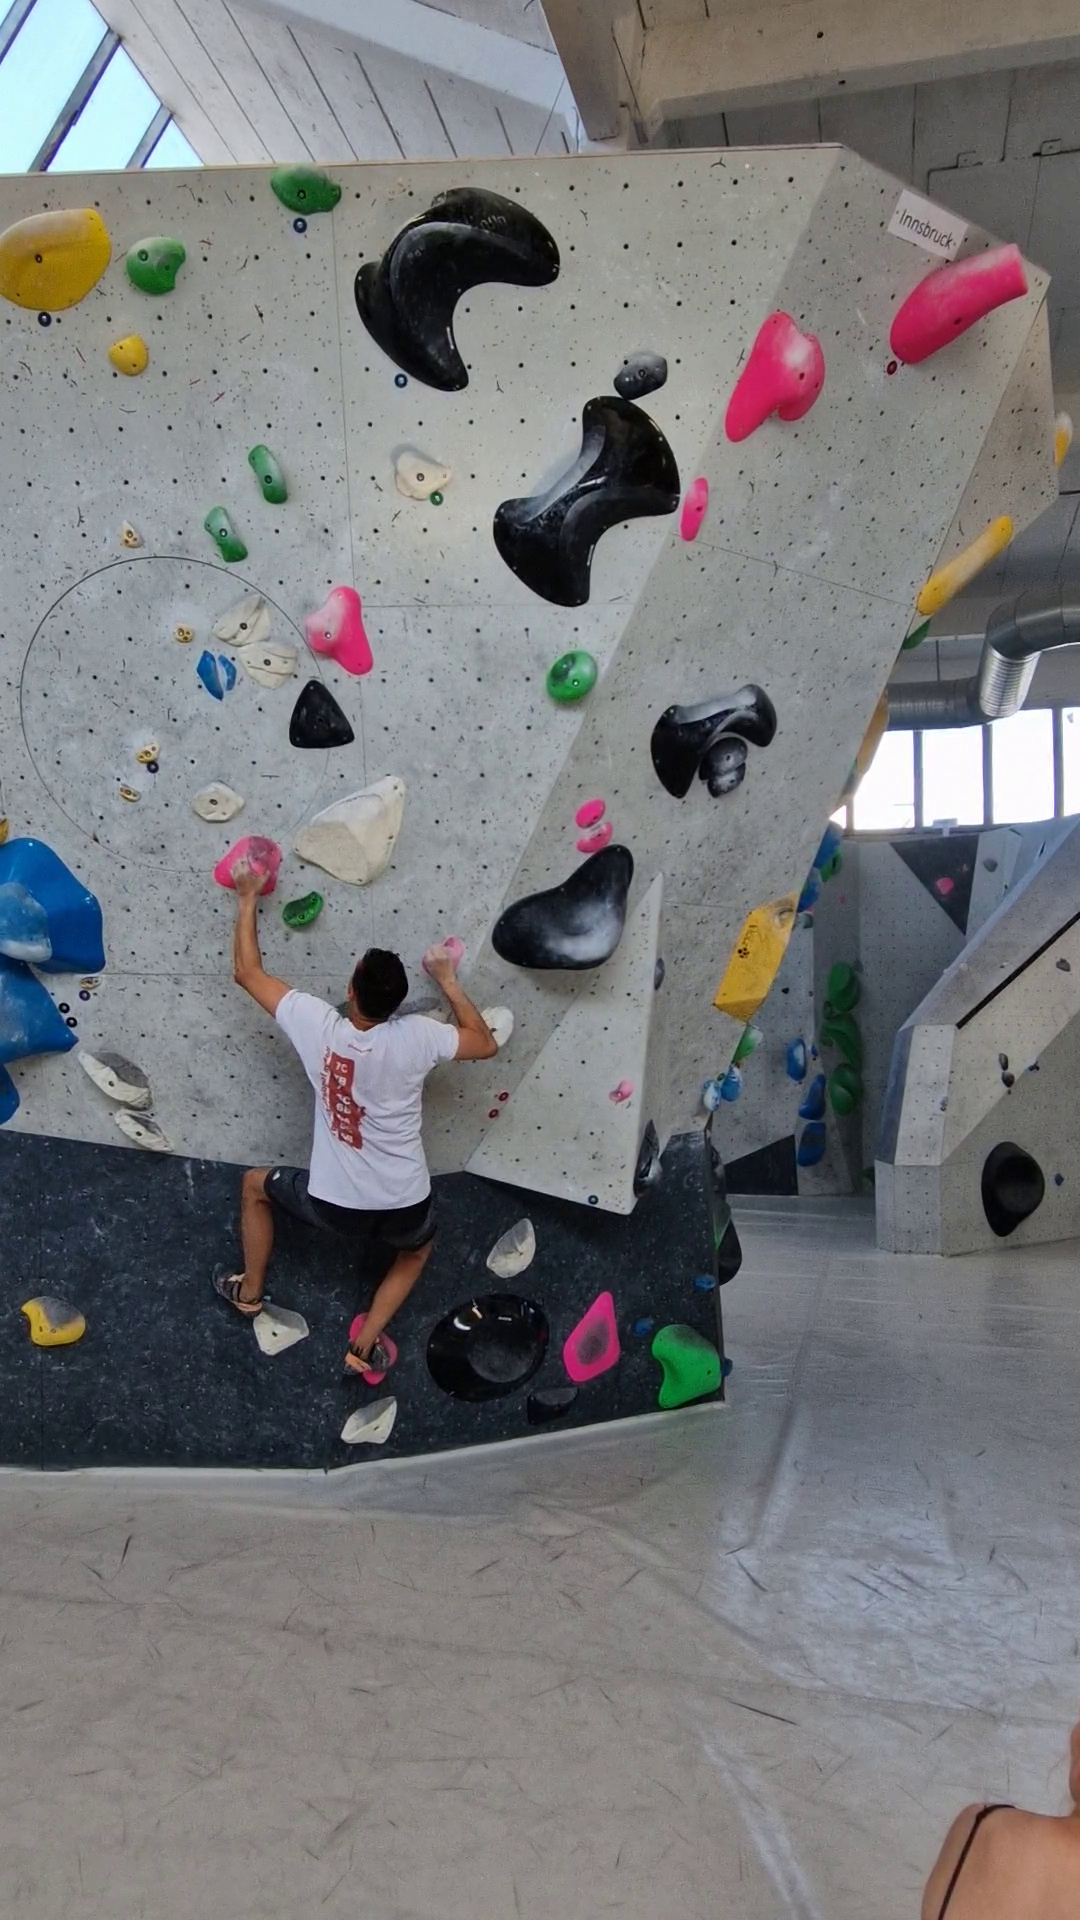
\includegraphics[width=\textwidth]{entities/CA_264.png}
        \caption{Frame 264}
    \end{subfigure}
    \begin{subfigure}{0.3\textwidth}
        \centering
        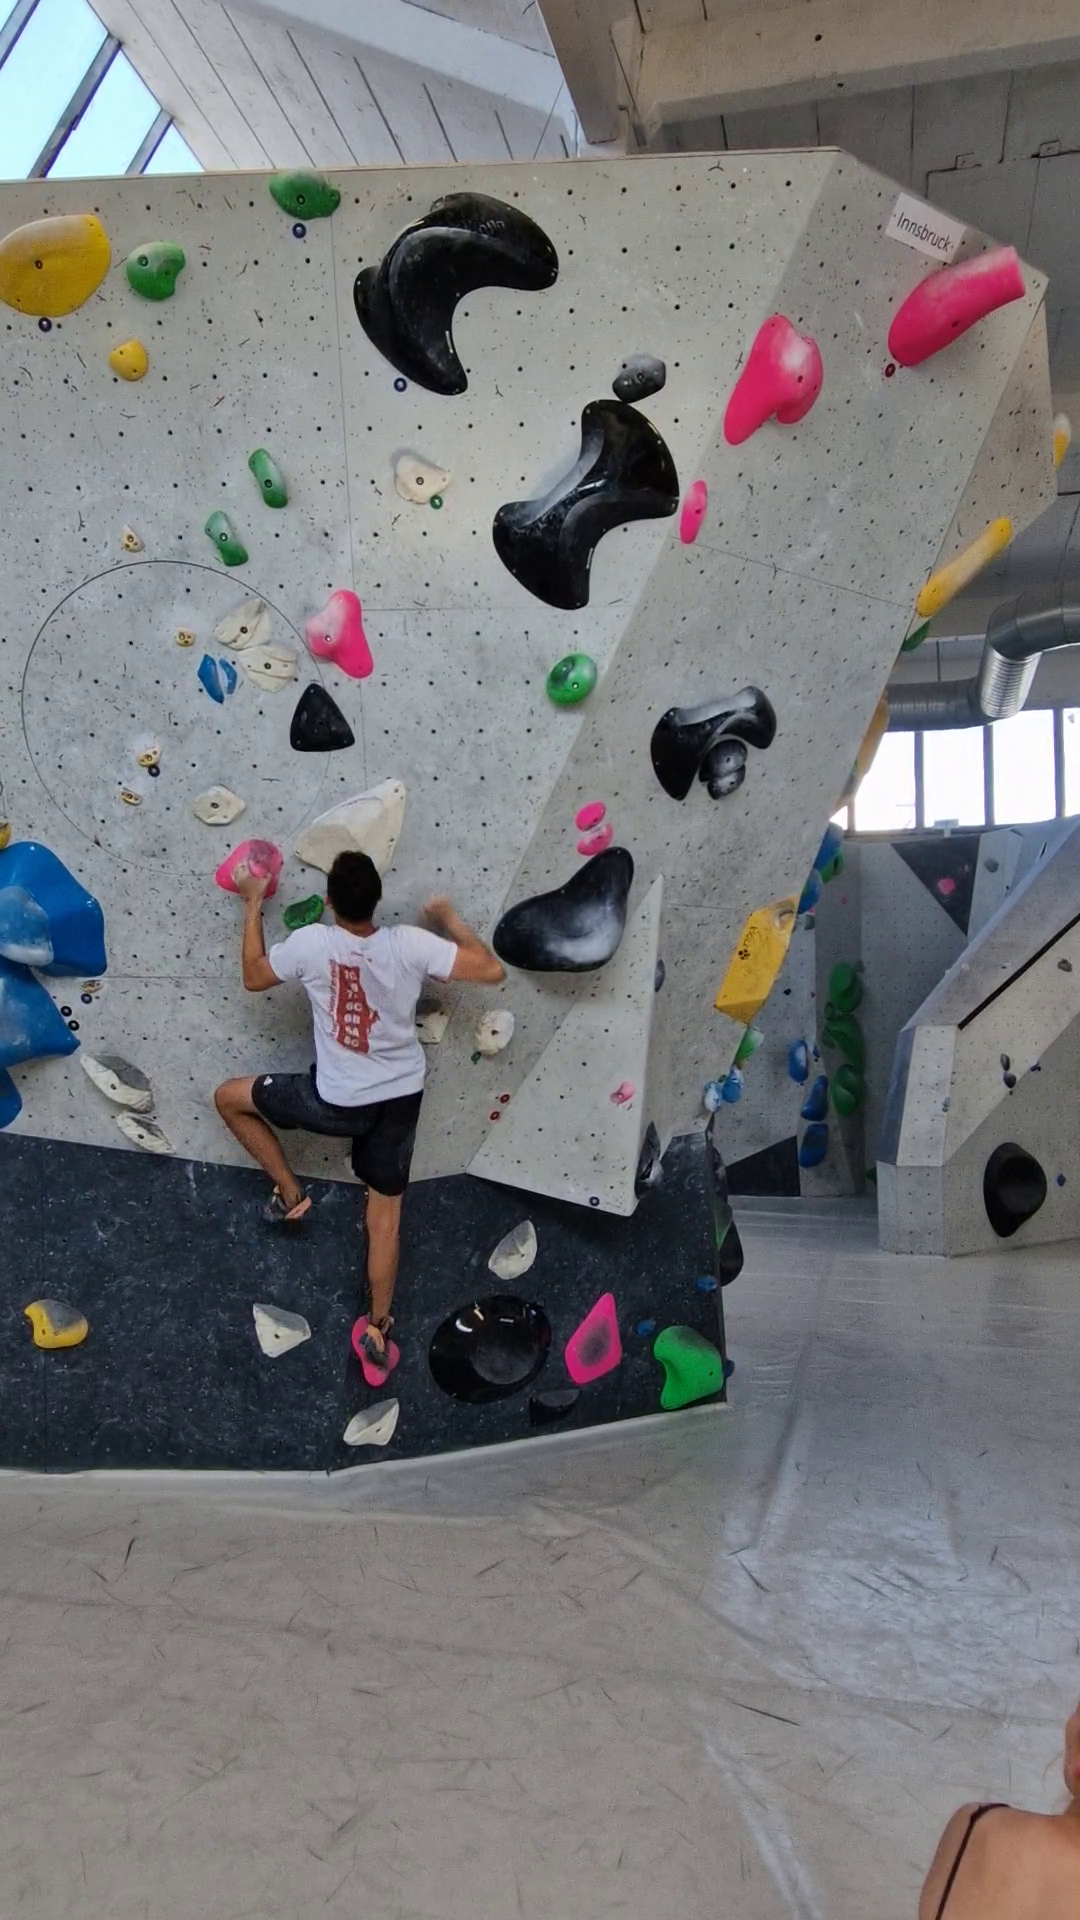
\includegraphics[width=\textwidth]{entities/CA_288.png}
        \caption{Frame 288}
    \end{subfigure}
    \begin{subfigure}{0.3\textwidth}
        \centering
        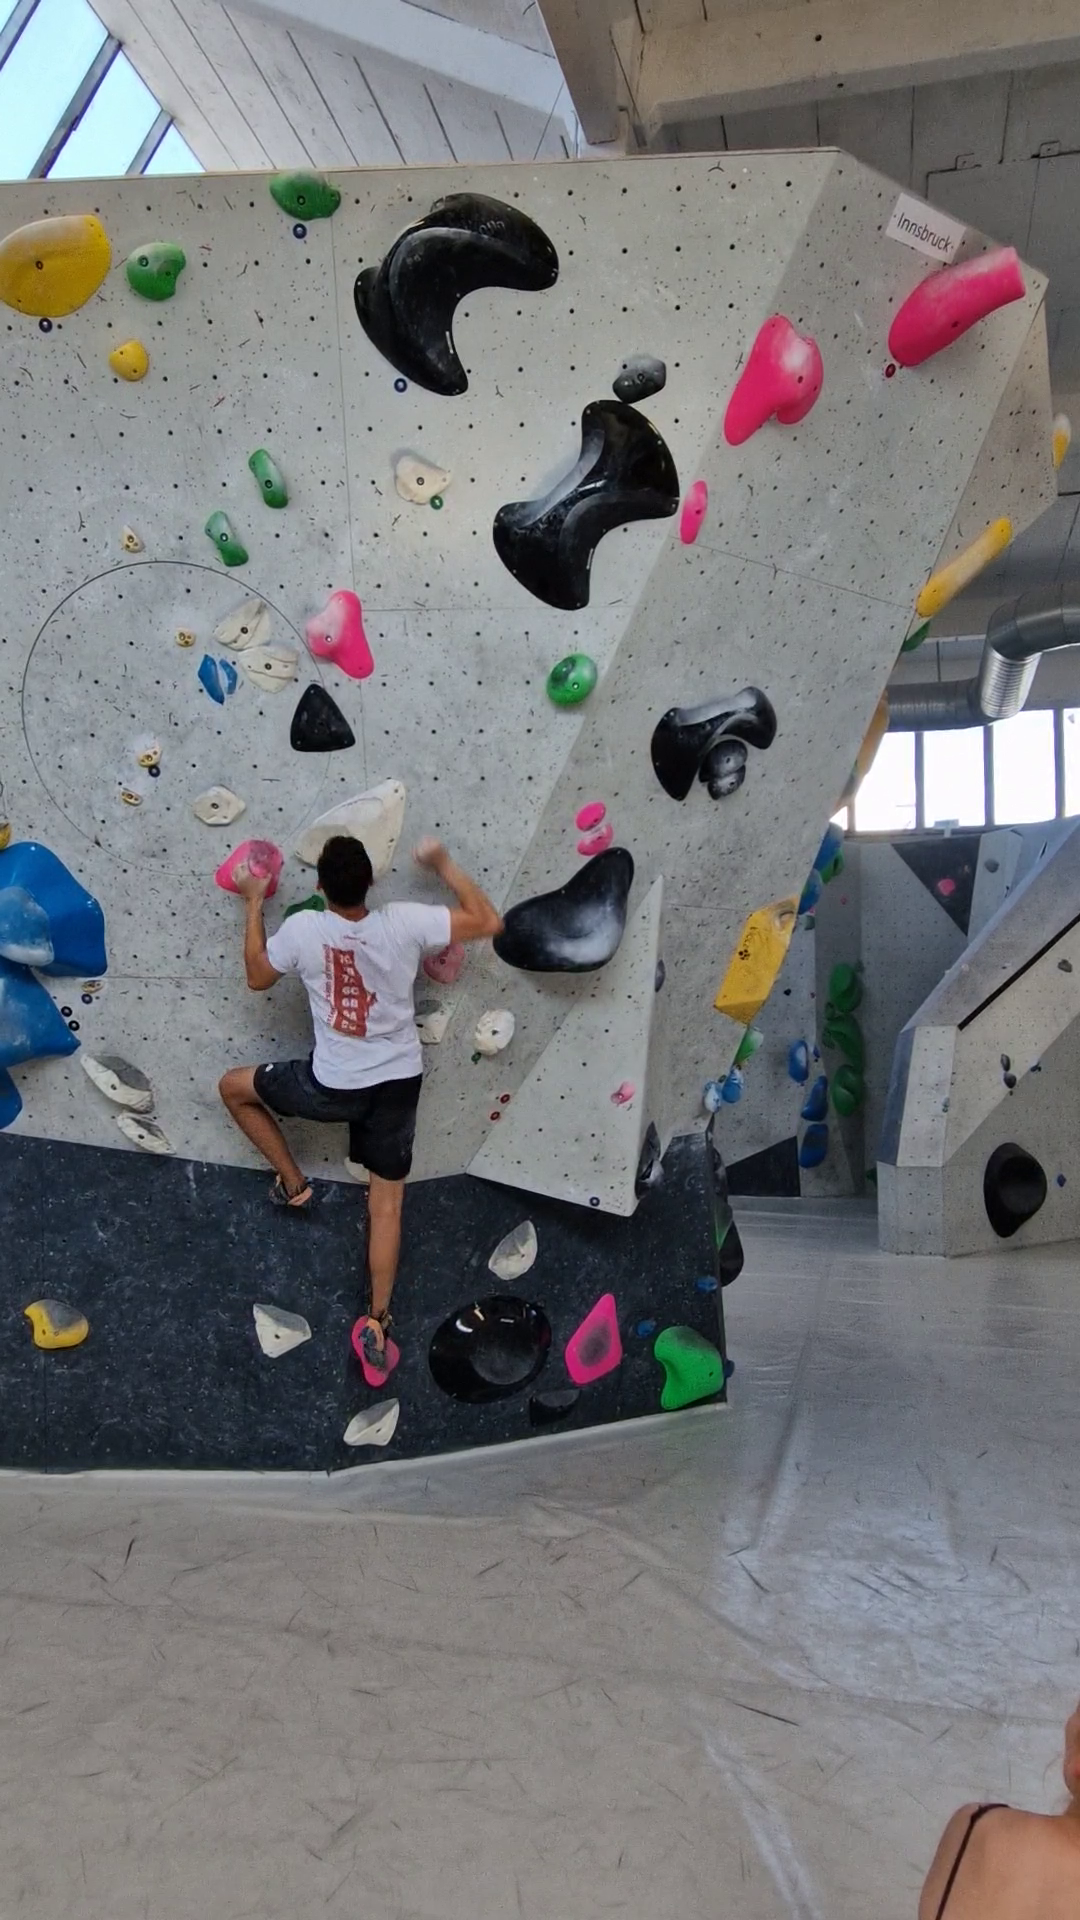
\includegraphics[width=\textwidth]{entities/CA_289.png}
        \caption{Frame 289}
    \end{subfigure}
    \begin{subfigure}{0.3\textwidth}
        \centering
        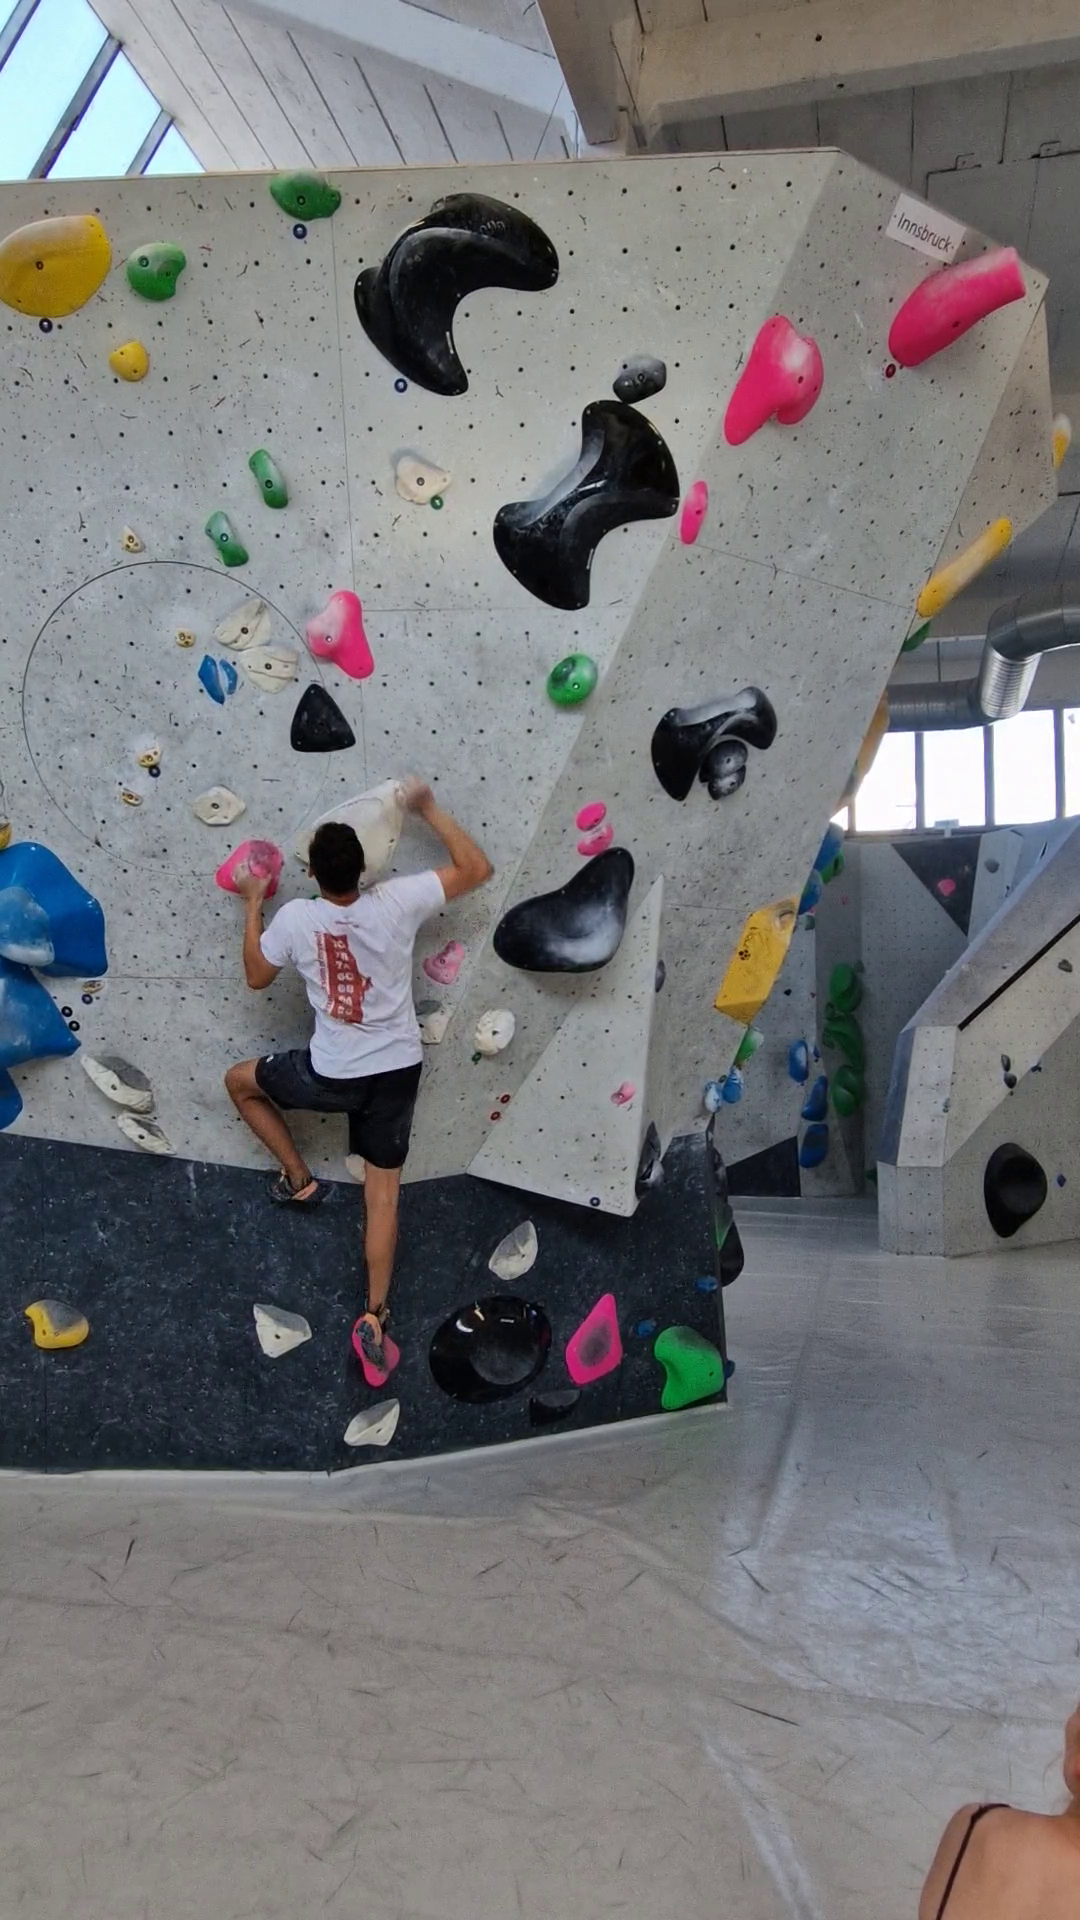
\includegraphics[width=\textwidth]{entities/CA_290.png}
        \caption{Frame 290}
    \end{subfigure}

    \caption{Example of two windows of three consecutive frames of a video from the ClimbAlong dataset}
    \label{fig:CA_dataset}
\end{figure}

As the aim of our models is to perform well on climbers, we will be using some annotated data of climbers. For this, ClimbAlong ApS has developed a dataset that we will be using. The dataset consists of videos various climbers on bouldering walls, where each video contains just a single climber. Figure \ref{fig:CA_dataset} illustrates two windows of consecutive frames of a single video from the ClimbAlong dataset. As shown in the figure, the videos in the dataset both contains static positions, where the climber holds a position for a while, as well as quick movemeents.
\\
\\
The ClimbAlong-dataset is split into two subsets. The first subset consists of $31$ fully annotated videos, where each annotation consists of $25$ keypoints. The second subset consists of $110$ fully annotated videos, where each annotation consists of $17$ keypoints. The two subsets have $13$ overlapping videos.
\\
\\
Each of the videos is in the RGB-format, is filmed in portrait mode with a resolution of $1080 \times 1920$ and $30$ frames per second. Table \ref{tab:keypoints} gives an overview of which keypoints are annotated in the two subsets. 

\subsection{The BRACE Dataset}
The second dataset we will be using is the \textit{BRACE} dataset \cite{BRACE}. We chose to use this dataset, as breakdancers tend to swap between static and acrobatic poses, similarly to the ones in the ClimbAlong dataset, making the poses relevant for our experiments in Section \ref{sec:experiments}.
\\
\\
This dataset consists of $1,352$ video sequences and a total of $334,538$ frames with keypoints annotations of breakdancers. The frames of the video sequences are in RGB and have a resolution of $1920 \times 1080$ \cite{BRACE}.
\\
\\
The frames of the video sequences have been annotated by initially using state-of-the-art human pose estimators to extract automatic poses. This was then followed by manually annotating bad keypoints, corresponding to difficult poses, as well as pose outliers. Finally, the automatic and manual annotations were merged, interpolating the keypoint seequence with Bézier curves. The keypoints is a list of 17-elements, following the COCO-format \cite{BRACE}.

\textbf{HVIS EKSEMPEL OG SKRIV NOGET OM HVILKE KEYPOITNS DER ER ANNOTERET}

\subsection{The Penn Action Dataset}
\begin{table}
    \begin{tabular}[htbp]{lllllllllllllll}
        \texttt{baseball\_pitch} & \texttt{baseball\_swing} & \texttt{bench\_press} \\
        \texttt{bowling} & \texttt{clean\_and\_jerk} & \texttt{golf\_swing} \\
        \texttt{jumping\_jacks} & \texttt{jump\_rope} & \texttt{pull\_ups} \\
        \texttt{push\_ups} & \texttt{sit\_ups} & \texttt{squats} \\
        \texttt{strumming\_guitar} & \texttt{tennis\_forehand} & \texttt{tennis\_serve}
    \end{tabular}
    \caption{The original $15$ action-types in the Penn Action dataset.}
    \label{tab:PA_actions}
\end{table}
The final dataset we will be using is the \textit{Penn Action} dataset \cite{penn_action}. This dataset consists of $2326$ video sequences of $15$ different action-types. Table \ref{tab:PA_actions} lists these $15$ action-types \cite{penn_action}.
\\
\\
Each sequence has been manually annotated with human joint annotation, consisting of $13$ joints as well as a corresponding binary visibility-flag for each joint. The frames of each sequence are in the RGB-format and has a resolution within the size of $640 \times 480$ \cite{penn_action}.
\\
\\
Unlike the BRACE dataset, most of the poses in the Penn Action dataset are not very acrobatic and thus are not very relevant for the poses of climbers. For that reason, we have decided to focus on the action-types that may contain more acrobatic poses. Thus, we only keep the sequences that have \texttt{baseball\_pitch}, \texttt{bench\_press} or \texttt{sit\_ups} as their corresponding action-type \cite{penn_action}.
\\
\\
\textbf{HVIS EKSEMPEL OG SKRIV NOGET OM HVILKE KEYPOITNS DER ER ANNOTERET}

\subsection{Preprocessing of the Data}

\subsection{The ClimbAlong Dataset}


\end{document}